\section{Introduction}

Work in recent years has demonstrated the efficacy of pretraining large and general foundation models \cite{bommasani2021opportunities} on noisy internet-scale datasets for use in downstream tasks in natural language \cite{devlin2018bert,liu2019roberta,raffel2019exploring,brown2020language} and computer vision. \cite{mahajan2018exploring, zhai2021scaling, radford2021learning}
For sequential decision domains (e.g.\ robotics, game playing, and computer usage) where agents must repeatedly act within an environment, a wealth of data also exists on the web; however, most of this data is in the form of \textit{unlabeled} video (i.e. without the actions taken at each frame), making it much less straightforward to train a behavioral prior in these domains than it is in e.g.\ natural language.
In a few rare settings, such as Chess, Go, and StarCraft, there already exist large datasets with action labels from various online platforms that researchers have used for imitation learning. \cite{silver2016mastering, vinyals2019grandmaster}
When large labeled datasets do not exist, the canonical strategy for training capable agents is reinforcement learning (RL),\cite{sutton2018reinforcement} which can be sample inefficient and expensive for hard-exploration problems.\cite{berner2019dota, baker2019emergent, jaderberg2019human, badia2020agent57, bellemare2016unifying, burda2018exploration, ecoffet2021first}
Many virtual tasks, e.g.\ navigating websites, using Photoshop, booking flights, etc., can be very hard to learn with RL and do not have large, commonly available sources of labeled data.\cite{humphreys2022data,pmlrv70shi17a}
In this paper, we seek to extend the paradigm of training large, general-purpose foundation models to sequential decision domains by utilizing freely available internet-scale unlabeled video datasets with a simple semi-supervised imitation learning method. We call this method Video PreTraining (VPT) and demonstrate its efficacy in the domain of Minecraft.

Existing semi-supervised imitation learning methods aim to learn with few or no explicit action labels; however, they generally rely on the policy's ability to explore the environment throughout training, making them susceptible to exploration bottlenecks. \cite{ng2000algorithms, torabi2019recent, ho2016generative, torabi2018behavioral, liu2018imitation}
Furthermore, most prior semi-supervised imitation learning work was tested in the relatively low data regime; because we experiment with \textit{far} more data ($\sim$70k hours of unlabeled video), we hypothesize that we can achieve good performance with a much simpler method, a trend that has proven true for pretraining in other modalities such as  text.\cite{brown2020language}
In particular, given a large but unlabeled dataset, we propose generating pseudo-labels by gathering a small amount of labeled data to train an inverse dynamics model (IDM) that predicts the action taken at each timestep in a video.
Behavioral cloning (BC) can require a large amount of data because the model must learn to infer intent and the distribution over future behaviors from only past observations.
In contrast, the inverse dynamics modeling task is simpler because it is \emph{non-causal}, meaning it can look at both past and future frames to infer actions.
In most settings, environment mechanics are far simpler than the breadth of human behavior that can take place within the environment, suggesting that non-causal IDMs could require far less data to train than causal BC models.
Using pseudo-labels generated from the IDM, we then train a model to mimic the distribution of behavior in the previously unlabeled dataset with standard behavioral cloning at scale, which does not require any model rollouts and thus does not suffer from any potential exploration bottlenecks in the environment.
Finally, we show we can fine-tune this model to downstream tasks with either behavioral cloning or reinforcement learning.

\begin{wrapfigure}{r}{0.33\textwidth}
\vspace{-20px}
\begin{center}
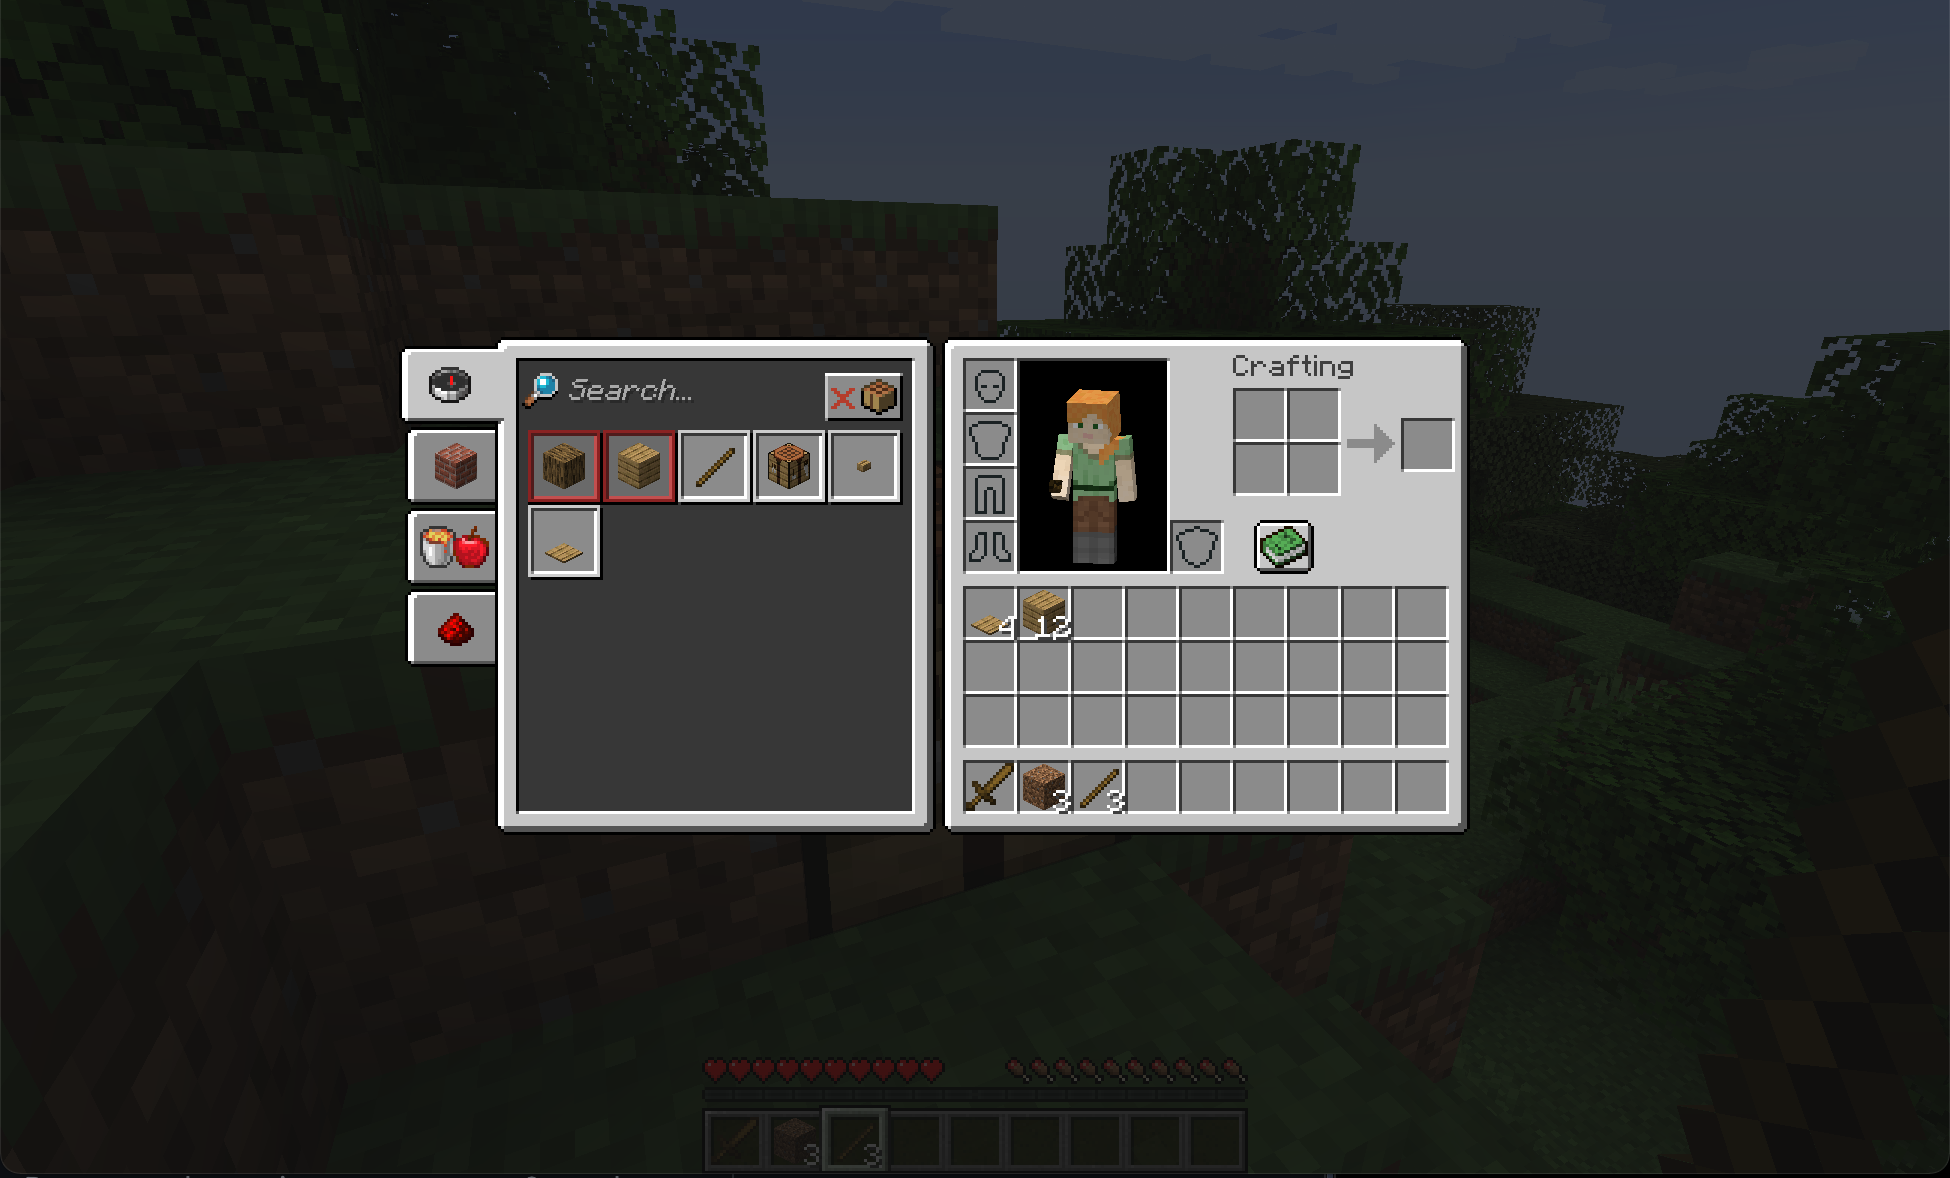
\includegraphics[width=\linewidth]{assets/crafting_screenshot.png} 
\end{center}
\vspace{-8px}
\caption{Example Minecraft crafting GUI. Agents use the mouse and keyboard to navigate menus and drag and drop items.
}
\label{fig:crafting_window}
\vspace{-10px}
\end{wrapfigure}
We chose to test our method in Minecraft because (a) it is one of the most actively played games in the world\cite{twinfinite2021played} and thus has a wealth of commonly available video data online, (b) it is a fairly open-ended sandbox game with an extremely wide variety of potential things to do, build, and collect, making our results more applicable to real-world applications such as computer usage, which also tends to be varied and open-ended, and (c) it has already garnered interest by the RL community as a research domain due to its complexity and correspondingly difficult exploration challenges.\cite{guss2019minerl, tessler2017deep, scheller2020sample, kanitscheider2021multi, oh2016control}
In this work we use the native human interface for Minecraft so that we can (1) most accurately model the human behavior distribution and reduce domain shift between video data and the environment, (2) make data collection easier by allowing our human contractors to play the game without modification, and (3) eliminate the need to hand-engineer a custom interface for models to interact with the environment.
This choice means that our models play at 20 frames per second and must use a mouse and keyboard interface to interact with human GUIs for crafting, smelting, trading, etc., including dragging items to specific slots or navigating the recipe book with the mouse cursor (Fig.~\ref{fig:crafting_window}).
Compared to prior work in Minecraft that uses a lower frame rate and constructs crafting and attacking macros,\cite{kanitscheider2021multi, patil2020align, skrynnik2020forgetful, lin2021juewu} using the native human interface drastically increases the environment's exploration difficulty, making most simple tasks near impossible with RL from scratch.
% which we validate in Sec.~\ref{section:results}.
Even the simple task of gathering a single wooden log while already facing a tree takes 60 consecutive attack actions with the human interface, meaning the chance for a naive random policy to succeed is $\frac{1}{2}^{60}$. While this paper shows results in Minecraft only, the VPT method is general and could be applied to any domain.


In Section \ref{section:results} we show that the VPT foundation model has nontrivial zero-shot performance, accomplishing tasks impossible to learn with RL alone, such as crafting planks and crafting tables (tasks requiring a human proficient in Minecraft a median of 50 seconds or $\sim$970 consecutive actions).
Through fine-tuning with behavioral cloning to smaller datasets that target more specific behavior distributions, our agent is able to push even further into the technology tree, crafting stone tools (taking a human a median of 2.3 minutes or $\sim$2790 actions).
Finally, fine-tuning via RL produces the most dramatic improvements: our agent is able to craft diamond tools, an unprecedented result in Minecraft made even more challenging by using the native human interface. This task requires a proficient human a median upwards of 20 minutes or $\sim$24000 actions.
The main contributions of this work are (1) we are the first to show promising results applying semi-supervised imitation learning to extremely large, noisy, and freely available video datasets for sequential decision domains, (2) we show that such pretraining plus fine-tuning enables agents to solve tasks that were otherwise impossible to learn, (3) we show that labeled contractor data is far more efficiently used within the VPT method than it would be by directly training a foundation model from it and (4) we open source our contractor data, trained model weights, and Minecraft environment for future research into learning to act via semi-supervised imitation learning at scale.